\documentclass{beamer}
%
% Choose how your presentation looks.
%
% For more themes, color themes and font themes, see:
% http://deic.uab.es/~iblanes/beamer_gallery/index_by_theme.html
%
\mode<presentation>
{
\usetheme{Madrid}      % Madrid, Montpellier, Pittsburgh, Rochester, boxes
\usecolortheme{seagull} 	% beaver, crane, dolphin, dove, lily, orchid, seagull, seahorse
\usefonttheme{default}  % or try serif, structurebold, ...
\setbeamertemplate{navigation symbols}{}
\setbeamertemplate{caption}[numbered]
}

\usepackage[portuguese]{babel}
\usepackage[utf8x]{inputenc}
\usepackage{multirow}
\usepackage{ragged2e}
\usepackage{textpos}
\usepackage[export]{adjustbox}
\justifying

\setlength{\parindent}{0.5cm}
%%%%%%%%%%%%%%%%%%%%%
% Títulos e etc
\title[Apresentação Semanal]{Tese de Mestrado}
\subtitle{Apresentação Semanal}
\author[M. Inocêncio]{Miguel Inocêncio}
\institute[UA]	{Universidade de Aveiro\\ 
				Instituto de Telecomunicações}
\date{23/04/2019}
\titlegraphic{
\includegraphics[height=1.5cm]{ua.jpg}\includegraphics[height=1.5cm]{IT.png}}

\begin{document}

%%%%%%%%%%%%%%%%%%%%%
% Página Inicial
\begin{frame}
	\titlepage
\end{frame}

%%%%%%%%%%%%%%%%%%%%%
% Table of Contents
\begin{frame}{Conteúdos}
	\tableofcontents
\end{frame}

%%%%%%%%%%%%%%%%%%%%%%
% Objetivos
\section{Objetivos}
\begin{frame}{Objetivos}
	\begin{itemize}
		\item Codificação de sequência de frames usando o software de referência
		\begin{itemize}
			\item Explorar opções de encoding
			\item Avaliar tempos de encoding
		\end{itemize}
		\item Visualização da sequência codificada
		\item Decode usando software de referência
		\begin{itemize}
			\item Explorar opções de decoding
			\item Avaliar tempos de decoding
		\end{itemize}		
		\item Teste com AOM Analyzer
	\end{itemize}
\end{frame}

%%%%%%%%%%%%%%%%%%%%%%
% Encoding
\section{Encoding}
\begin{frame}{Encoding}

	A \textit{Alliance for open media} diponibiliza todas as ferramentas de encoding e decoding, assim como algumas soluções para encode e decode.
	
	\begin{columns}
		\begin{column}[T, onlytextwidth]{.45\textwidth}%
			\begin{itemize}
				\setlength\itemsep{3cm}
				\item Tools para construção de encoder/decoder custom 
				\item Encoder/Decoder com ferramentas acima
			\end{itemize}
		\end{column}
		\begin{column}[T]{.45\textwidth}%
			\begin{figure}				
				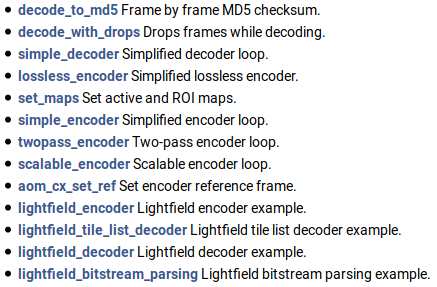
\includegraphics[height=3cm,left]{tools.png}\\
				\vspace{0.75cm}
				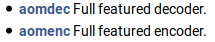
\includegraphics[height=0.5cm,left]{full.png}
			\end{figure}			
		\end{column}		
	\end{columns}	
\end{frame}

\begin{frame}{Encoding}
	Para o teste básico de encoding, foi usada uma secção da sequência \textit{"Paris"}:
	\begin{itemize}
		\item $288 \times 352$
		\item 10 frames
		\item 4:2:0
	\end{itemize}
	
	O encoder foi feito com o \textit{aomenc}, com apenas uma passagem, ao contrário do default (2). Mesmo assim, o teste demorou cerca de 10 horas a concluir.
\end{frame}

%%%%%%%%%%%%%%%%%%%%%%
% Decoding/Visualização
\section{Decoding/Visualização}
\begin{frame}
	\frametitle{Decoding/Visualização}

	Para descodificação da sequência, foram usadas várias abordagens:

	\begin{enumerate}
		\item Ferramentas integradas do Firefox
		\item \textit{AOMAnalyzer} --- ferramenta da AOM
		\item \textit{aomdec}
	\end{enumerate}

	Todas as ferramentas fizeram o decode com sucesso.

	A ferramenta que permite uma análise mais detalhada trata-se do analisador personalizado para o AV1.
\end{frame}

\begin{frame}
	\frametitle{AOMAnalyzer}

	Ferramenta de análise intensiva para o bit stream gerado na codificação.

	\begin{figure}
		\centering
		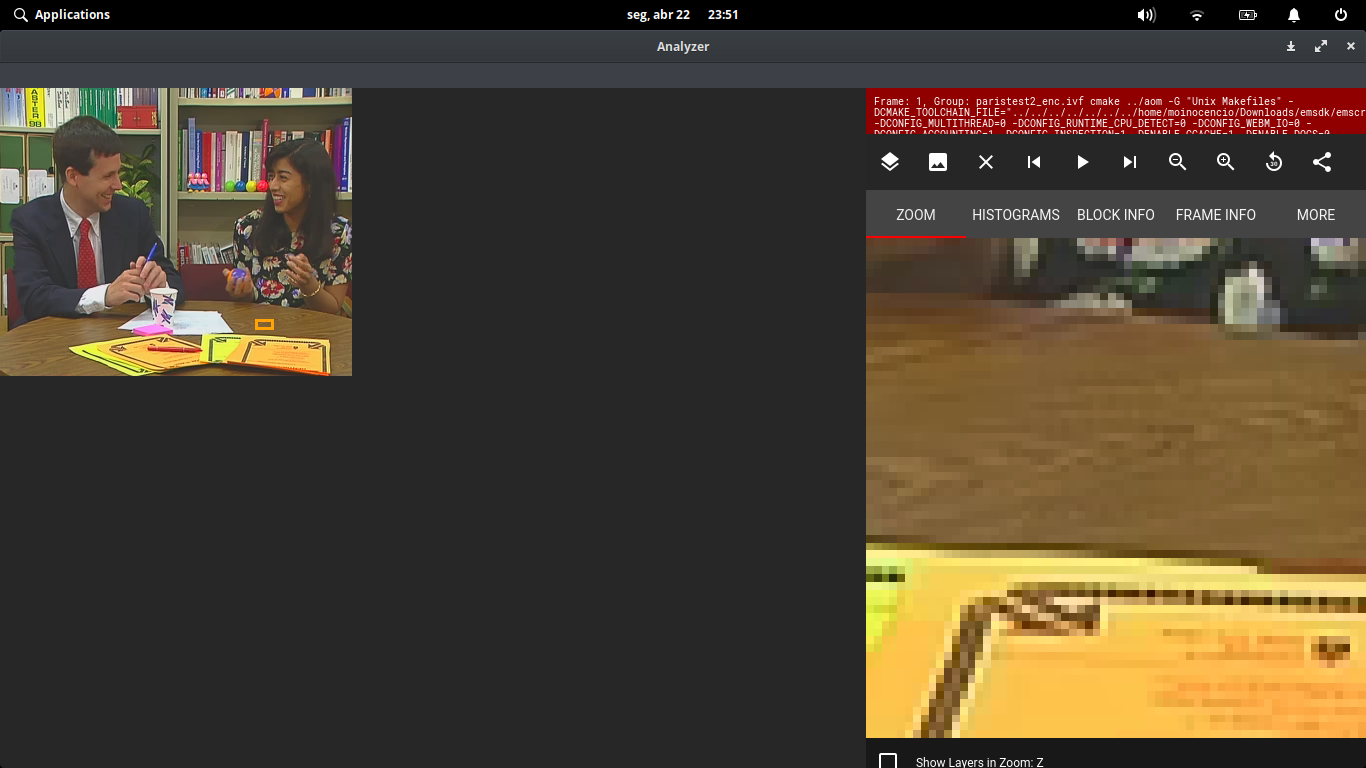
\includegraphics[height=6cm]{aomanal.png}
	\end{figure}
\end{frame}


\end{document}